\section{Unsharpen Mask}
\subsection{Defining and applying the Unsharpen Effect}
Applying this filter counterintuativley has the effect of sharpening the image. We first begin by passing the image $I$ through a low pass filter to get $I_l$. This can then be subtracted fro m $I$ to leave us with a new image that only contains the high frequency components in this image. We can then apply a gain of $\alpha$ to this image to control how much of the high frequency components we want to add back to the image. This then gives us our final shapened image. If we raise $\alpha$ too much, we end up introducing sharpening artifacts to the image. However, if $\alpha$ is too small we dont end up with the desired sharpening effects. This is demonstrated in Figure \ref{fig:SharpenedImages}.

\begin{figure}[!h]
    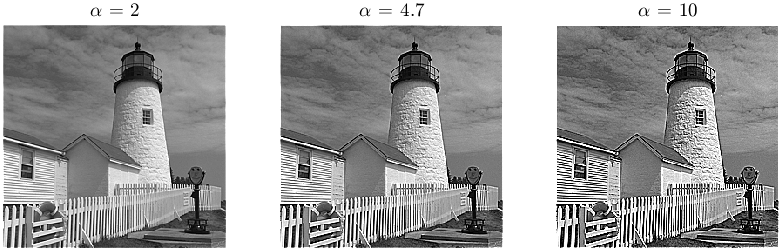
\includegraphics[width=1\textwidth]{SharpenedImages.png}
    \centering
    \caption{Sharpening effect with 3 values of $\alpha$}
    \label{fig:SharpenedImages}
\end{figure}

\noindent Through trial and error I found that an $\alpha$ value of 4.7 provideed good enough sharpening results without introducing too many artifacts. These artifacts are visible in the 3rd image as banding on the wall of the house and on the fence.